% fig-g2delta: G2 train-holdout remedy (2x2)
% Data: R/g2delta_*.csv → out/g2delta-*.tex
%
% Chrome (jointmon-style pt offsets, not axis-relative legend@1.xx):
%   titles @ 1.015 — tight to the axis top; panel letters on this row in the gutter
%   c/d legends — TikZ nodes @34pt above axis.north (south-anchored); clears titles
%   a/b shared legend — TikZ node @26pt above the a/b midline
%   a/b row @ 3.20in — clears c/d legend tops (~2.94) + a/b rotated x-labels
% Panel-d legend is a TikZ node (not pgfplots ybar legend — tall samples collided).
\documentclass[border=2pt]{standalone}
% inspect_style.tex: Shared style definitions for all Inspect figures
% Enforces uniform fonts, colors, and panel label positioning

\usepackage[T1]{fontenc}
\usepackage{lmodern}  % Latin Modern for Type 1 fonts
\usepackage{amssymb}  % \blacksquare for shared legends
\usepackage{pgfplots}
\usepackage{pgfplotstable}
\pgfplotsset{compat=1.18}

% Color palette (Okabe-Ito colorblind-safe, print-safe)
% -- Backbones (used wherever PatchCore vs Dinomaly are distinguished)
\definecolor{cPatchcore}{HTML}{0072B2}   % blue
\definecolor{cDinomaly}{HTML}{D55E00}    % vermillion
% -- Decision classes / gates
\definecolor{cAccept}{HTML}{009E73}      % green
\definecolor{cDefer}{HTML}{E69F00}       % orange
\definecolor{cReject}{HTML}{D55E00}      % red
\definecolor{cControl}{HTML}{56B4E9}     % light blue
\definecolor{cTransfer}{HTML}{CC79A7}    % pink
% -- Benchmarks (canonical palette; used wherever MVTec/VisA/MPDD are
%    distinguished, so benchmark colouring is uniform across all figures and
%    never collides with the backbone blue/vermillion above)
\definecolor{cMVTecAD}{HTML}{0072B2}     % blue
\definecolor{cVisA}{HTML}{E69F00}        % orange
\definecolor{cMPDD}{HTML}{009E73}        % green

% Typography defaults
\newcommand{\figfont}{\fontsize{8}{9.5}\selectfont}
\newcommand{\axislabelfont}{\fontsize{9}{10}\selectfont}
\newcommand{\titlefont}{\fontsize{9}{10}\selectfont}
\newcommand{\tickfont}{\fontsize{7}{8}\selectfont}
\newcommand{\panellabelfont}{\fontsize{9}{10}\selectfont\bfseries}

% Panel label OUTSIDE the axis (axis clip would otherwise swallow it).
% Usage after \end{axis}: \panellabel{axname}{a}
% Parked in the left gutter at the top of the axis frame — NOT on the
% title baseline — so titles can stay truly centered over the plot box.
\newcommand{\panellabel}[2]{%
  \node[anchor=south east, font=\panellabelfont, inner sep=0.5pt]
    at ([xshift=-8pt, yshift=7pt] #1.north west) {\textbf{#2}};%
}

% Standard axis styles. Titles centered above the plot box only.
\pgfplotsset{
  inspect/centertitle/.style={
    title style={at={(0.5,1.10)}, anchor=south, font=\titlefont},
  },
  inspect default/.style={
    axis x line=bottom,
    axis y line=left,
    xlabel style={font=\axislabelfont},
    ylabel style={font=\axislabelfont},
    inspect/centertitle,
    x tick label style={font=\tickfont},
    y tick label style={font=\tickfont},
    legend style={font=\tickfont, draw=none, fill=none},
  }
}


\definecolor{cCertified}{HTML}{009E73}
\definecolor{cRefuseFloor}{HTML}{999999}
\definecolor{cRefuseKS}{HTML}{E69F00}
\definecolor{cGate}{HTML}{0072B2}

% Letter on the title row, parked in the left gutter (south-east → sits left of NW).
% Name must not start with \g<digit> (TeX accent primitive).
\newcommand{\gtwolabel}[2]{\panellabelshift{#1}{#2}{-12pt}{10pt}}

\begin{document}
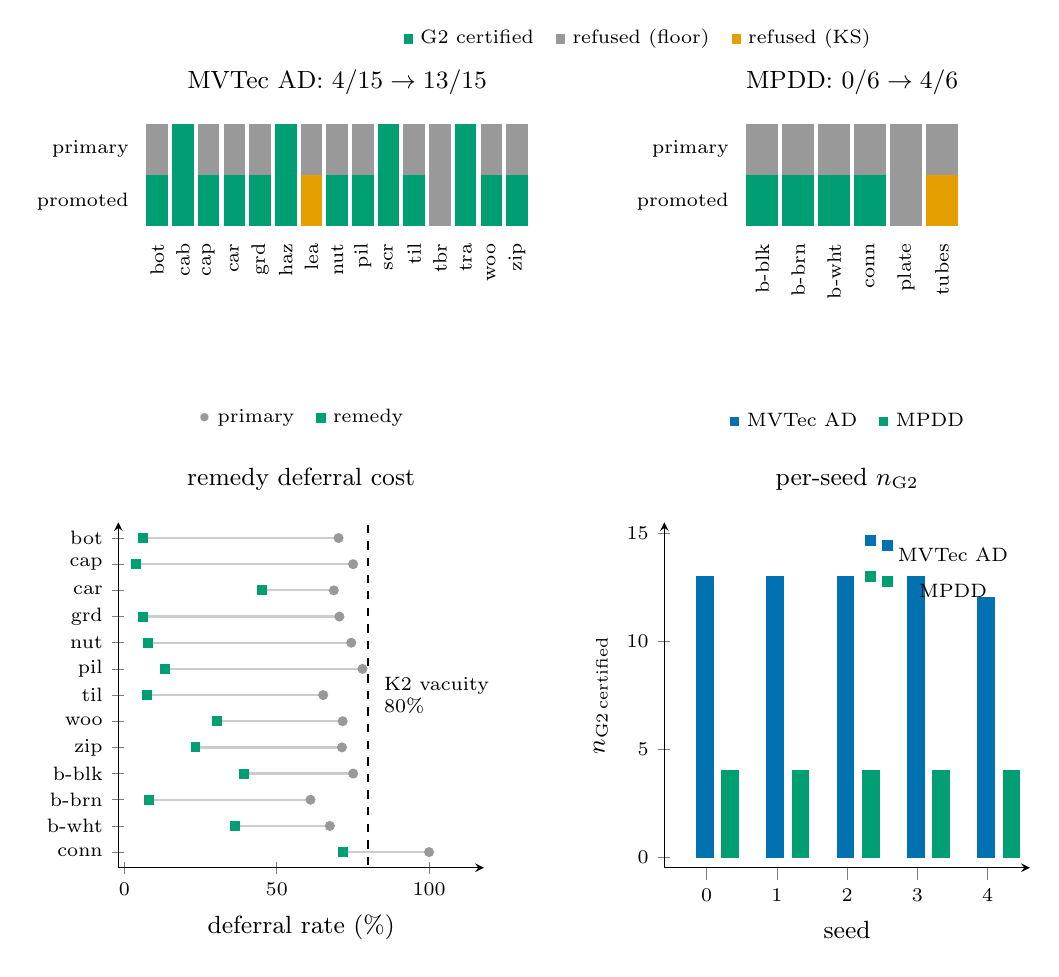
\begin{tikzpicture}[font=\figfont]
\gdef\GtwoDeltaCYtick{0,1,2,3,4,5,6,7,8,9,10,11,12}
\gdef\GtwoDeltaCYticklabels{conn,b-wht,b-brn,b-blk,zip,woo,til,pil,nut,grd,car,cap,bot}
\gdef\GtwoDeltaCN{13}


\pgfplotsset{
  g2/title near axis/.style={
    title style={at={(0.5,1.015)}, anchor=south, font=\titlefont, text=black},
  },
}

% Panel a: MVTec tiles
% a/b at 3.20in: c/d north=2.35; c/d legend south@34pt≈2.82; top≈2.96;
% ~0.24in left for a/b rotated x-labels hanging into the row gutter.
\begin{axis}[
  inspect default,
  name=axa, width=2.55in, height=1.15in, at={(0.55in,3.20in)},
  xmin=0, xmax=15, ymin=0, ymax=2,
  xtick={0.5,1.5,2.5,3.5,4.5,5.5,6.5,7.5,8.5,9.5,10.5,11.5,12.5,13.5,14.5},
  xticklabels={bot,cab,cap,car,grd,haz,lea,nut,pil,scr,til,tbr,tra,woo,zip},
  x tick label style={font=\tickfont, rotate=90, anchor=east},
  ytick={0.5,1.5}, yticklabels={promoted,primary},
  axis line style={draw=none},
  tick style={draw=none},
  g2/title near axis,
  title={MVTec AD: $4/15\to13/15$},
  clip=false,
]
\begin{scope}[shift={(0,0)}]
  % generated by process_g2delta.R
\fill[cCertified] (0,0) rectangle ++(1,1);
\fill[cRefuseFloor] (0,1) rectangle ++(1,1);
\draw[white, line width=1.5pt] (0,0) rectangle ++(1,2);
\fill[cCertified] (1,0) rectangle ++(1,1);
\fill[cCertified] (1,1) rectangle ++(1,1);
\draw[white, line width=1.5pt] (1,0) rectangle ++(1,2);
\fill[cCertified] (2,0) rectangle ++(1,1);
\fill[cRefuseFloor] (2,1) rectangle ++(1,1);
\draw[white, line width=1.5pt] (2,0) rectangle ++(1,2);
\fill[cCertified] (3,0) rectangle ++(1,1);
\fill[cRefuseFloor] (3,1) rectangle ++(1,1);
\draw[white, line width=1.5pt] (3,0) rectangle ++(1,2);
\fill[cCertified] (4,0) rectangle ++(1,1);
\fill[cRefuseFloor] (4,1) rectangle ++(1,1);
\draw[white, line width=1.5pt] (4,0) rectangle ++(1,2);
\fill[cCertified] (5,0) rectangle ++(1,1);
\fill[cCertified] (5,1) rectangle ++(1,1);
\draw[white, line width=1.5pt] (5,0) rectangle ++(1,2);
\fill[cRefuseKS] (6,0) rectangle ++(1,1);
\fill[cRefuseFloor] (6,1) rectangle ++(1,1);
\draw[white, line width=1.5pt] (6,0) rectangle ++(1,2);
\fill[cCertified] (7,0) rectangle ++(1,1);
\fill[cRefuseFloor] (7,1) rectangle ++(1,1);
\draw[white, line width=1.5pt] (7,0) rectangle ++(1,2);
\fill[cCertified] (8,0) rectangle ++(1,1);
\fill[cRefuseFloor] (8,1) rectangle ++(1,1);
\draw[white, line width=1.5pt] (8,0) rectangle ++(1,2);
\fill[cCertified] (9,0) rectangle ++(1,1);
\fill[cCertified] (9,1) rectangle ++(1,1);
\draw[white, line width=1.5pt] (9,0) rectangle ++(1,2);
\fill[cCertified] (10,0) rectangle ++(1,1);
\fill[cRefuseFloor] (10,1) rectangle ++(1,1);
\draw[white, line width=1.5pt] (10,0) rectangle ++(1,2);
\fill[cRefuseFloor] (11,0) rectangle ++(1,1);
\fill[cRefuseFloor] (11,1) rectangle ++(1,1);
\draw[white, line width=1.5pt] (11,0) rectangle ++(1,2);
\fill[cCertified] (12,0) rectangle ++(1,1);
\fill[cCertified] (12,1) rectangle ++(1,1);
\draw[white, line width=1.5pt] (12,0) rectangle ++(1,2);
\fill[cCertified] (13,0) rectangle ++(1,1);
\fill[cRefuseFloor] (13,1) rectangle ++(1,1);
\draw[white, line width=1.5pt] (13,0) rectangle ++(1,2);
\fill[cCertified] (14,0) rectangle ++(1,1);
\fill[cRefuseFloor] (14,1) rectangle ++(1,1);
\draw[white, line width=1.5pt] (14,0) rectangle ++(1,2);

\end{scope}
\end{axis}
\gtwolabel{axa}{a}

% Panel b: MPDD tiles
\begin{axis}[
  inspect default,
  name=axb, width=1.70in, height=1.15in, at={(3.55in,3.20in)},
  xmin=0, xmax=6, ymin=0, ymax=2,
  xtick={0.5,1.5,2.5,3.5,4.5,5.5},
  xticklabels={b-blk,b-brn,b-wht,conn,plate,tubes},
  x tick label style={font=\tickfont, rotate=90, anchor=east},
  ytick={0.5,1.5}, yticklabels={promoted,primary},
  axis line style={draw=none},
  tick style={draw=none},
  g2/title near axis,
  title={MPDD: $0/6\to4/6$},
  clip=false,
]
\begin{scope}
  % generated by process_g2delta.R
\fill[cCertified] (0,0) rectangle ++(1,1);
\fill[cRefuseFloor] (0,1) rectangle ++(1,1);
\draw[white, line width=1.5pt] (0,0) rectangle ++(1,2);
\fill[cCertified] (1,0) rectangle ++(1,1);
\fill[cRefuseFloor] (1,1) rectangle ++(1,1);
\draw[white, line width=1.5pt] (1,0) rectangle ++(1,2);
\fill[cCertified] (2,0) rectangle ++(1,1);
\fill[cRefuseFloor] (2,1) rectangle ++(1,1);
\draw[white, line width=1.5pt] (2,0) rectangle ++(1,2);
\fill[cCertified] (3,0) rectangle ++(1,1);
\fill[cRefuseFloor] (3,1) rectangle ++(1,1);
\draw[white, line width=1.5pt] (3,0) rectangle ++(1,2);
\fill[cRefuseFloor] (4,0) rectangle ++(1,1);
\fill[cRefuseFloor] (4,1) rectangle ++(1,1);
\draw[white, line width=1.5pt] (4,0) rectangle ++(1,2);
\fill[cRefuseKS] (5,0) rectangle ++(1,1);
\fill[cRefuseFloor] (5,1) rectangle ++(1,1);
\draw[white, line width=1.5pt] (5,0) rectangle ++(1,2);

\end{scope}
\end{axis}
\gtwolabel{axb}{b}

% Shared tile legend — 26pt south-anchor clears title tops (~10pt) with ~8pt air.
\path (axa.north east) -- (axb.north west) coordinate[midway] (abmid);
\node[anchor=south, font=\tickfont, text=black, inner sep=0.5pt]
  at ([yshift=26pt]abmid) {%
  {\color{cCertified}\rule{1.1ex}{1.1ex}}~G2 certified\quad
  {\color{cRefuseFloor}\rule{1.1ex}{1.1ex}}~refused (floor)\quad
  {\color{cRefuseKS}\rule{1.1ex}{1.1ex}}~refused (KS)%
};

% Panel c: remedy deferral — ytick labels expanded from meta macros
\begin{axis}[
  inspect default,
  name=axc, width=2.45in, height=2.35in, at={(0.42in,0)},
  xmin=-2, xmax=118,
  ymin=-0.6, ymax=\GtwoDeltaCN-0.4,
  xlabel={deferral rate (\%)},
  ytick={\GtwoDeltaCYtick},
  yticklabels/.expanded={\GtwoDeltaCYticklabels},
  g2/title near axis,
  title={remedy deferral cost},
  clip=false,
]
% generated by process_g2delta.R -- panel c
\draw[black!20, line width=0.8pt] (axis cs:6.07,12) -- (axis cs:70.29,12);
\addplot[cRefuseFloor, only marks, mark=*, mark size=1.6pt, forget plot] coordinates {(70.29,12)};
\addplot[cCertified, only marks, mark=square*, mark size=1.6pt, forget plot] coordinates {(6.07,12)};
\draw[black!20, line width=0.8pt] (axis cs:3.89,11) -- (axis cs:75.06,11);
\addplot[cRefuseFloor, only marks, mark=*, mark size=1.6pt, forget plot] coordinates {(75.06,11)};
\addplot[cCertified, only marks, mark=square*, mark size=1.6pt, forget plot] coordinates {(3.89,11)};
\draw[black!20, line width=0.8pt] (axis cs:45.20,10) -- (axis cs:68.73,10);
\addplot[cRefuseFloor, only marks, mark=*, mark size=1.6pt, forget plot] coordinates {(68.73,10)};
\addplot[cCertified, only marks, mark=square*, mark size=1.6pt, forget plot] coordinates {(45.20,10)};
\draw[black!20, line width=0.8pt] (axis cs:6.10,9) -- (axis cs:70.57,9);
\addplot[cRefuseFloor, only marks, mark=*, mark size=1.6pt, forget plot] coordinates {(70.57,9)};
\addplot[cCertified, only marks, mark=square*, mark size=1.6pt, forget plot] coordinates {(6.10,9)};
\draw[black!20, line width=0.8pt] (axis cs:7.71,8) -- (axis cs:74.47,8);
\addplot[cRefuseFloor, only marks, mark=*, mark size=1.6pt, forget plot] coordinates {(74.47,8)};
\addplot[cCertified, only marks, mark=square*, mark size=1.6pt, forget plot] coordinates {(7.71,8)};
\draw[black!20, line width=0.8pt] (axis cs:13.29,7) -- (axis cs:78.15,7);
\addplot[cRefuseFloor, only marks, mark=*, mark size=1.6pt, forget plot] coordinates {(78.15,7)};
\addplot[cCertified, only marks, mark=square*, mark size=1.6pt, forget plot] coordinates {(13.29,7)};
\draw[black!20, line width=0.8pt] (axis cs:7.53,6) -- (axis cs:65.25,6);
\addplot[cRefuseFloor, only marks, mark=*, mark size=1.6pt, forget plot] coordinates {(65.25,6)};
\addplot[cCertified, only marks, mark=square*, mark size=1.6pt, forget plot] coordinates {(7.53,6)};
\draw[black!20, line width=0.8pt] (axis cs:30.36,5) -- (axis cs:71.64,5);
\addplot[cRefuseFloor, only marks, mark=*, mark size=1.6pt, forget plot] coordinates {(71.64,5)};
\addplot[cCertified, only marks, mark=square*, mark size=1.6pt, forget plot] coordinates {(30.36,5)};
\draw[black!20, line width=0.8pt] (axis cs:23.32,4) -- (axis cs:71.41,4);
\addplot[cRefuseFloor, only marks, mark=*, mark size=1.6pt, forget plot] coordinates {(71.41,4)};
\addplot[cCertified, only marks, mark=square*, mark size=1.6pt, forget plot] coordinates {(23.32,4)};
\draw[black!20, line width=0.8pt] (axis cs:39.28,3) -- (axis cs:75.08,3);
\addplot[cRefuseFloor, only marks, mark=*, mark size=1.6pt, forget plot] coordinates {(75.08,3)};
\addplot[cCertified, only marks, mark=square*, mark size=1.6pt, forget plot] coordinates {(39.28,3)};
\draw[black!20, line width=0.8pt] (axis cs:8.13,2) -- (axis cs:61.08,2);
\addplot[cRefuseFloor, only marks, mark=*, mark size=1.6pt, forget plot] coordinates {(61.08,2)};
\addplot[cCertified, only marks, mark=square*, mark size=1.6pt, forget plot] coordinates {(8.13,2)};
\draw[black!20, line width=0.8pt] (axis cs:36.23,1) -- (axis cs:67.43,1);
\addplot[cRefuseFloor, only marks, mark=*, mark size=1.6pt, forget plot] coordinates {(67.43,1)};
\addplot[cCertified, only marks, mark=square*, mark size=1.6pt, forget plot] coordinates {(36.23,1)};
\draw[black!20, line width=0.8pt] (axis cs:71.73,0) -- (axis cs:100.00,0);
\addplot[cRefuseFloor, only marks, mark=*, mark size=1.6pt, forget plot] coordinates {(100.00,0)};
\addplot[cCertified, only marks, mark=square*, mark size=1.6pt, forget plot] coordinates {(71.73,0)};
\draw[black, dashed, line width=0.8pt] (axis cs:80,-0.5) -- (axis cs:80,12.5);
\node[anchor=west, font=\tickfont, text=black, align=left] at (axis cs:82,6.00) {K2 vacuity\\80\%};

\end{axis}
\gtwolabel{axc}{c}
% Legend as TikZ node (not pgfplots) — same 34pt offset as a/b shared key.
\node[anchor=south, font=\tickfont, text=black, inner sep=0.5pt]
  at ([yshift=34pt] axc.north) {%
  {\color{cRefuseFloor}$\bullet$}~primary\quad
  {\color{cCertified}\rule{1.1ex}{1.1ex}}~remedy%
};

% Panel d: per-seed n_G2
\begin{axis}[
  inspect default,
  name=axd, width=2.45in, height=2.35in, at={(3.15in,0)},
  ybar=2pt, bar width=6pt,
  xmin=-0.6, xmax=4.6, ymin=-0.5, ymax=15.5,
  xlabel={seed},
  ylabel={$n_{\mathrm{G2\,certified}}$},
  xtick={0,1,2,3,4},
  g2/title near axis,
  title={per-seed $n_{\mathrm{G2}}$},
  clip=false,
]
% generated by process_g2delta.R -- panel d
\addlegendimage{cGate, only marks, mark=square*, mark size=1.8pt}
\addlegendentry{MVTec AD}
\addlegendimage{cAccept, only marks, mark=square*, mark size=1.8pt}
\addlegendentry{MPDD}
\addplot[cGate, fill=cGate, forget plot] coordinates {(-0.18,13.00) (0.82,13.00) (1.82,13.00) (2.82,13.00) (3.82,12.00)};
\addplot[cAccept, fill=cAccept, forget plot] coordinates {(0.18,4.00) (1.18,4.00) (2.18,4.00) (3.18,4.00) (4.18,4.00)};

\end{axis}
\gtwolabel{axd}{d}
% Flat-square TikZ legend — avoids ybar's tall pgfplots legend samples colliding
% with the title (the previous legend@1.16 + ybar image height stacked on title).
\node[anchor=south, font=\tickfont, text=black, inner sep=0.5pt]
  at ([yshift=34pt] axd.north) {%
  {\color{cGate}\rule{1.1ex}{1.1ex}}~MVTec AD\quad
  {\color{cAccept}\rule{1.1ex}{1.1ex}}~MPDD%
};

\end{tikzpicture}
\end{document}
